\documentclass[a4paper,10pt]{article}
\usepackage[left=2cm, right=2cm, top=1cm, bottom=2cm]{geometry}
\usepackage{enumitem, hyperref}
\usepackage{fontawesome5}
\usepackage{tabularx}
\usepackage{ltablex}
\usepackage{tikz}
\usepackage{graphicx}
\usepackage{lmodern, titlesec}
\usepackage{parskip}
\usepackage{bold-extra}  % Enables bold small caps
\usepackage{tcolorbox}
\usepackage{ebgaramond}
\usepackage{xcolor}
\usetikzlibrary{calc,decorations.pathmorphing}

% Option A: vertical Euler identity (simple, classy)
\newcommand{\EulerRail}{%
	
\begin{tikzpicture}[baseline]
		\node[rotate=90, text=gray!60, inner sep=0pt] {$\displaystyle e^{i\pi}+1=0$};
	\end{tikzpicture}%
}

% Option B: tiny sine-wave sparkline
\newcommand{\SineRail}{%
	\begin{tikzpicture}[baseline,x=0.18cm,y=0.18cm]
		\begin{scope}[rotate=90]
			\draw[gray!60, line width=0.4pt, domain=0:6.283, samples=80]
			plot (\x, {0.8*sin(\x r)});
		\end{scope}
	\end{tikzpicture}%
}

% Option C: zeta/basel identity
\newcommand{\BaselRail}{%
	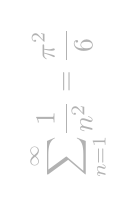
\begin{tikzpicture}[baseline]
		\node[rotate=90, text=gray!60, inner sep=0pt] {$\displaystyle \sum_{n=1}^{\infty}\!\frac{1}{n^2}=\frac{\pi^2}{6}$};
	\end{tikzpicture}%
}

% Tikz Libraries
\usetikzlibrary{mindmap,shadows,shadings}

% Define colors
\definecolor{burnt}{HTML}{913b01}
\definecolor{tealshade}{HTML}{bfdfdf}
\definecolor{burntshade}{HTML}{FFE0CF}

\titleformat{\section}
{\Large\bfseries\scshape\color{burnt}}  % Bold + Small Caps + Teal
{} % No numbering
{0pt} % No spacing
{} % No title prefix
[\vspace{0.1cm} \titlerule] % Adds spacing & horizontal rule

\keepXColumns

\renewcommand{\baselinestretch}{1.1}
\renewcommand{\labelitemi}{\textbullet}
\newcommand{\refnum}[2]{\href{#1}{\textbf{[#2]}}}
\newcommand{\sep}{\;\;}
\newcommand{\module}[2]{\makebox[2cm][l]{\textbf{#1}} #2}

\hypersetup{
	colorlinks=true,
	linkcolor=teal,
	filecolor=teal,
	urlcolor=teal,
	citecolor=teal
}

\begin{document}
\begin{center}
	{\Huge\textbf{\textsc{\textcolor{burnt}{Henri Branken}}}}\\[0.5cm]
\end{center}

\begin{tcolorbox}[
	colback=teal!10, % Light gray background
	colframe=teal,   % Teal border
	boxrule=1pt, % Border thickness
	width=\textwidth,
	left=10pt, right=10pt, % Padding inside the box
	sharp corners=northwest
	]
	\begin{center}
		\faHome~ \textbf{Potchefstroom (2531), South Africa} \quad \faEnvelope~ \href{mailto:henri.branken777@gmail.com}{\textbf{henri.branken777@gmail.com}} \quad\\ \faPhone~ \textbf{+27 (0) 82 785 5983} \quad \faGithub~ \href{https://github.com/HenriBranken}{\textbf{GitHub}}
	\end{center}
\end{tcolorbox}

% === Career Objective Box ===
\begin{tcolorbox}[
	colback=burntshade,
	colframe=burnt,
	boxrule=1pt,
	sharp corners=northwest,
	rounded corners=southwest,
	coltitle=white,
	fonttitle=\large\bfseries\scshape,
	title=Current Workplace,
	width=\textwidth,
	left=10pt, right=10pt, top=5pt, bottom=5pt
	]
	Eduvos
\end{tcolorbox}

% \quad \faLinkedin~ \href{https://www.linkedin.com/in/henri-branken-1423a2153/}{\textbf{LinkedIn}}

\section*{Overview}
I hold an MSc in Space Physics (\textit{cum laude}), which has equipped me with strong research training and proficiency in mathematical analysis and modeling. I subsequently spent approximately 3.5 years as a Data Scientist at Matogen Applied Insights, where I delivered a portfolio performance monitor and a credit-loss model for a telecommunications client, a Power BI dashboard for monitoring agricultural nutrient distributions, and a model to predict grape harvest dates.

To broaden my software-engineering skill set, I completed the HyperionDev bootcamp, working with HTML, CSS, JavaScript, the MERN stack, and Java—strengthening my full-stack development and database management capabilities. After completion, I served as a HyperionDev Coding Mentor (July~2024--March~2025). I currently lecture IT modules at Eduvos (Potchefstroom Campus). Teaching keeps me in a cycle of continual learning and curriculum refinement, ensuring I remain current with emerging tools and practices.

My data-science background has made me comfortable with back-end systems and data-driven applications, and I value full-stack development for its balance of analytical rigor and creative problem-solving. While fluent in Windows environments, I also work extensively in open-source ecosystems, particularly Linux~\faLinux{\vspace*{2pt}}


\begin{center}	
	{\fontsize{11}{10}\selectfont\textcolor{burnt}{\faHandPointRight} Here is a \href{https://coalition-fed.onrender.com/}{\textbf{\underline{FrontEnd Demo}}} that showcases my skills in ReactJS, Express \& SCSS \href{https://github.com/HenriBranken/coalition-fed}{\textcolor{teal}{\faGithub}}}.\\Also check out my \href{https://expense-tracker-five-sepia.vercel.app/}{\textbf{\underline{Expense Tracking App}}}, which is a fullstack app I built using the SvelteKit Framework \href{https://github.com/HenriBranken/expense-tracker}{\textcolor{teal}{\faGithub}}
\end{center}

\section*{Experience}
\renewcommand{\arraystretch}{1.1}
\begin{tabularx}{\textwidth}{r l X}
	    \textbf{2025/04--Current} & 
	\multicolumn{2}{| l}{\textbf{\href{https://www.eduvos.com/}{\textsc{Eduvos}}} IT Lecturer, Potchefstroom Campus, 
		\href{mailto:henri.branken@eduvos.com}{\textbf{henri.branken@eduvos.com}}} \\
		
	& \multicolumn{1}{| l}{\textbullet} & \module{CODAA2}{PowerBI for Data Analytics} \\
	& \multicolumn{1}{| l}{\textbullet} & \module{ITTNA3}{4th Industrial Revolution} \\
	& \multicolumn{1}{| l}{\textbullet} & \module{ITMRA2}{Mathematics for Robotics} \\
	& \multicolumn{1}{| l}{\textbullet} & \module{ITISA1}{Introduction to Information Systems} \\
	& \multicolumn{1}{| l}{\textbullet} & \module{ITSCA2}{Scientific Computing in Python} \\
	& \multicolumn{1}{| l}{\textbullet} & \module{ITMCA1}{Maths for Computing (Extra Classes)} \\
	& \multicolumn{1}{| l}{\textbullet} & \module{ITMTA1}{Mathematics 1A (Differentiation)} \\
	& \multicolumn{1}{| l}{\textbullet} & \module{ITDPA2}{Data Structures and Algorithms in Python} \\
	& \multicolumn{1}{| l}{\textbullet} & \module{ITMLA2}{Machine Learning Algorithms} \\
	& \multicolumn{1}{| l}{\textbullet} & \module{ITMTB1}{Mathematics 1B (Integration)} \\
	& \multicolumn{1}{| l}{\textbullet} & \module{ITOOA3}{Object Oriented System's Analysis and Design}\\
	& \multicolumn{1}{| l}{\textbullet} & \module{ITECA3}{Web Development and E-Commerce}\\
	& \multicolumn{1}{| l}{\textbullet} & \module{ITSKA1}{Computer Literacy Skills}\\
	& & \\[-5pt]
	
	\textbf{2024/07--2025/03} & \multicolumn{2}{| l}{\textbf{\href{https://www.hyperiondev.com/}{HyperionDev}} Code Reviewer \& Student Mentor.} \\
	& \multicolumn{1}{| l}{\textbullet} & As a Coding Mentor, I evaluated students' coding submissions for tasks and provided constructive feedback to enhance the quality, efficiency, and styling of their code. Additionally, I conducted live sessions to provide personalised guidance, helping students effectively tackle specific tasks and develop their programming skills. \\
	& \multicolumn{1}{| l}{\textbullet} & Acted as an SME to refactor \href{https://github.com/HenriBranken/AcademicPortfolio/blob/main/Testing\_a\_React\_App.pdf}{\textbf{Task Contents}} for the course syllabus.\\
	& \multicolumn{1}{|l}{\textbullet} & Conducted an \href{https://github.com/HenriBranken/AcademicPortfolio/blob/main/Academic\%20Onboarding\%20Session.pdf}{\textbf{onboarding session}} for newly-enrolled students on the \href{https://livestorm.co/}{\textbf{LiveStorm}} platform. \\
	& \multicolumn{1}{|l}{\textbullet} & Please see my full Academic Portfolio \href{https://github.com/HenriBranken/AcademicPortfolio?tab=readme-ov-file\#academic-portfolio}{\textbf{here}}. \\
	& & \\[-5pt]
		
	\textbf{2022/12} & \multicolumn{2}{| X}{The completion of my own \href{https://drive.google.com/file/d/1tkuLPdXlgsDundxbjZLjyl6aZhKUqDid/view?usp=sharing}{\textbf{Japanese Language Studies book}} (typeset in \href{https://en.wikipedia.org/wiki/LaTeX}{\textbf{\LaTeX}}), which took 4+ years. Without a doubt, this is the project I’m most proud of!} \\
	& & \\[-5pt]
	
	\textbf{2019--2022/07} & \multicolumn{2}{| X}{\textbf{Data Scientist} at \href{https://ai.matogen.com/}{\textbf{Matogen Applied Insights}}.} \\
	& \multicolumn{1}{| l}{\textbullet} & Built PowerBI Dashboard to monitor Nutrient Distributions of Farm Crops.\\
	& \multicolumn{1}{| l}{\textbullet} & Built Tableau Dashboards for a Debt Counseling Company to closely track agent performance.\\
	& \multicolumn{1}{| l}{\textbullet} & Interrogated the \href{https://hcup-us.ahrq.gov/nisoverview.jsp}{\textbf{Nationwide Inpatient Sample (NIS)}} to determine factors influencing mortality rates in patients receiving orthopedic procedures.\\
	& \multicolumn{1}{| l}{\textbullet} & Built an AI Model to improve the accuracy of harvest-date predictions for grape cultivars.\\
	& \multicolumn{1}{| l}{\textbullet} & Built a Portfolio Performance Monitor and Expected Credit Loss Model for a Telco Company based on Service Line Age Files and Bureau Data.  Here are \href{https://github.com/henri-branken-matogen/henri_libs}{\textbf{PySpark Libraries}} I translated from SAS.\\
	& \multicolumn{1}{| l}{\textbullet} & Made a \href{https://github.com/HenriBranken/ProbeSchedule}{\textbf{Python Algorithm}} to compute accurate Water Irrigation Schedules for Farm Crops based on telemetry readings and weather forecasts.  This was to improve on the crude method of setting water irrigation parameters based on season of the year.\\
	& & \\[-5pt]
	
	\textbf{2017} & \multicolumn{2}{| X}{Internship at the \href{https://natural-sciences.nwu.ac.za/space-research}{\textbf{Centre for Space Research, Potchefstroom}.}} \\
	& & \\ [-5pt]

	\textbf{2011} & \multicolumn{2}{| X}{\href{https://github.com/HenriBranken/Henri_Branken_Certification/blob/master/tertiary/Supplemental_Instruction_Leader.pdf}{\textbf{Supplemental Instruction Leader}} for the 2011 Term in Mathematics (1\textsuperscript{st} year level).} \\[-5pt]
\end{tabularx}
A list of references can be provided upon request.

\section*{Education \& Training}
\renewcommand{\arraystretch}{1.1}
\begin{tabularx}{\textwidth}{r l X}
	\textbf{2023/01--2023/09} & \multicolumn{2}{| l}{\textbf{\href{https://www.hyperiondev.com/bootcamps/immersive/full-stack-web-and-software-engineer/}{HyperionDev Full Stack Web \& Software Engineer Bootcamp}} (Student).}\\
	& \multicolumn{1}{| l}{\textbullet} & HyperionDev is accredited with the \textbf{\href{https://www.mict.org.za/}{MICT Seta}} (ACC/2017/05/0005). This course bears \textbf{30 Credits}, aligned to an \textbf{NQF Level 5 Qualification}. \\
	& \multicolumn{1}{| l}{\textbullet} & Please click on this \href{https://www.hyperiondev.com/portfolio/79331/}{\textbf{link}} to view my entire HyperionDev Profile.\\
	& \multicolumn{1}{| l}{\textbullet} & Received a \href{https://www.facebook.com/henri.branken.9/posts/pfbid02gUh1H3ovPTfn4TLrr3ZYFWzhcEyuDte2xsZTLbPjHiNZStTRPEArNnius6T5Bj5rl}{\textbf{\textit{Student of the Month} Award}} for my commitment to excellence and continuous improvement.\\
	& \multicolumn{1}{| l}{\textbullet} & \textbf{Noteworthy GitHub Repos:} \refnum{https://github.com/HenriBranken/react\_hangman\#hangman-game-in-react}{1} Hangman Game \textit{(React UI)} \refnum{https://github.com/HenriBranken/ReactDictionaryUsage\#dictionary-app}{2} Dictionary App \textit{(Interacting with 3rd-Party API)} \refnum{https://github.com/HenriBranken/github\_app\#github-web-app}{3} GitHub API App \textit{(Express, React, Axios)} \refnum{https://github.com/HenriBranken/CoolTech\#cooltech-credential-management-system}{4} Credential Management System \textit{(Authentication, Authorization, JWT)} \refnum{https://github.com/HenriBranken/FoodQuick\#food-ordering-program-capstone}{5} Delivery App \textit{(Java OOP)} \refnum{https://github.com/HenriBranken/PoisePMS\#poise-project-management-system-pms}{6} Project Management System \textit{(Java, JDBC, MySQL)} \refnum{https://github.com/HenriBranken/ISS\#international-space-station-iss}{7} International Space Station \textit{(Asynchronous JavaScript)} \refnum{https://github.com/HenriBranken/montyHall\#the-monty-hall-problem}{8} Monty Hall Game \textit{(React, State Management)} \refnum{https://henribranken.github.io/MyCV/}{9} FrontEnd UI \textit{(HTML, SCSS)} \\
	& & \\[-5pt]
	
	\textbf{2022/08--2022/12} & \multicolumn{1}{| l}{\textbullet} &
	\textbf{\href{https://github.com/HenriBranken/Henri_Branken_Certification/blob/master/online_courses/TEFL_Certificate.pdf}{Qualifi Level 5 Diploma in Teaching English as a Foreign Language (The TEFL Academy)}}. \\
	& \multicolumn{1}{| l}{\textbullet} & \href{https://github.com/HenriBranken/Henri_Branken_Certification/blob/master/online_courses/TEFL_20hour_certificate.pdf}{\textbf{Classroom TEFL Course Certificate (20 Hours)}} \\
	& \multicolumn{1}{| l}{\textbullet} & TEFL, Teaching Business English (30 Hours) \\
	& \multicolumn{1}{| l}{\textbullet} & The completion of my own \href{https://drive.google.com/file/d/1tkuLPdXlgsDundxbjZLjyl6aZhKUqDid/view?usp=sharing}{\textbf{Japanese Language Studies book}} (typeset in \href{https://en.wikipedia.org/wiki/LaTeX}{\textbf{\LaTeX}}), which took 4+ years. Without a doubt, this is the project I’m most proud of! \\
	& & \\[-5pt]
	
	\textbf{2018} & \multicolumn{1}{| l}{\textbullet} & Completed \href{https://github.com/HenriBranken/Henri\_Branken\_Certification?tab=readme-ov-file\#online-courses-completed-at-datacamp-in-alphabetical-order}{\textbf{Online Courses}}
	at \textbf{\href{https://www.udemy.com/}{Udemy}} and \textbf{\href{https://www.datacamp.com/}{DataCamp}} with a strong focus on \textbf{Python Data Science} and \textbf{Linux Essentials}. \\
	& \multicolumn{1}{| l}{\textbullet} & Attended \textbf{\href{https://2018.za.pycon.org/}{PyConZA 2018}} in Johannesburg.\\
	& & \\[-5pt]
	
	\textbf{2017} & \multicolumn{1}{| l}{\textbullet} & Completed the \textbf{``Data Science with Python'' Track} on DataCamp \href{https://github.com/HenriBranken/Henri_Branken_Certification/blob/master/online_courses/datacamp_dot_com/datacamp_Data_Scientist_with_Python_Track.pdf}{\textbf{(Certificate Number \#13,897)}}.\\
	& \multicolumn{1}{| l}{\textbullet} & Completed the 2017 \textbf{\href{https://adventofcode.com/}{Advent of Code}} challenges. My Python solutions may be viewed in this \href{https://github.com/HenriBranken/Advent_of_Code_2017_python_3}{\textbf{repo}.} \\
	& & \\[-5pt]
	
	\textbf{2014--2016} & \multicolumn{2}{| X}{\textbf{Master of Science in \textsc{Space Physics}, \href{https://www.nwu.ac.za/}{North-West University}, Potchefstroom}.}\\
	& \multicolumn{2}{| X}{\textsc{Dissertation:} \href{https://repository.nwu.ac.za/handle/10394/25063}{\textit{\textbf{Weighing dark matter in brightest cluster galaxies}}}}\\
	& \multicolumn{2}{| X}{\textsc{Supervisor:} Prof. Ilani Loubser} \\
	& \multicolumn{2}{| X}{\textsc{Avg. Score:} 85\%, \textit{Cum Laude}} \\
	& \multicolumn{2}{| X}{Awarded as the top achiever on Master’s level in the Centre for Space Research (for the year 2016).} \\
	& \multicolumn{2}{| X}{\href{https://github.com/HenriBranken/Henri_Branken_Certification/blob/master/tertiary/full_university_academic_record.pdf}{\textbf{Academic Transcript}}} \\
	& & \\[-5pt]
	
	\textbf{2013} & \multicolumn{2}{| X}{\textbf{Honours Bachelor of Science in \textsc{Physics}, \href{https://www.nwu.ac.za/}{North-West University}, Potchefstroom}.}\\
	& \multicolumn{2}{| X}{\textsc{Avg. Score:} 92\%, \textit{Cum Laude}}\\
	& \multicolumn{2}{| X}{Awarded as the Top Achiever in Honours in Physics.}\\
	& & \\[-5pt]
	
	\textbf{2010--2012} & \multicolumn{2}{| X}{\textbf{Bachelor of Science in \textsc{Physical and Chemical Sciences}, \href{https://www.nwu.ac.za/}{North-West University}, Potchefstroom}.} \\
	& \multicolumn{2}{| X}{Majored in \textbf{Physics and Applied Mathematics}} \\
	& \multicolumn{2}{| X}{\textsc{3rd Year Avg. Score:} 95\%, \textit{Cum Laude}} \\
	& \multicolumn{1}{| l}{\textbullet} & Awarded as the top achiever in the 1\textsuperscript{st}, 2\textsuperscript{nd}, and 3\textsuperscript{rd} years of the Physics curriculum.\\
	& \multicolumn{1}{| l}{\textbullet} & Awarded as the top student in the Faculty of Natural Sciences for the 1\textsuperscript{st} and 3\textsuperscript{rd} years of study.\\
	& & \\[-5pt]
	
	\textbf{2009} & \multicolumn{2}{|X}{\textbf{Matriculated with 8 distinctions from St. Andrew’s Private School, Welkom}} \\
	& \multicolumn{2}{|X}{\href{https://github.com/HenriBranken/Henri\_Branken\_Certification/blob/master/secondary/National\_Senior\_Certificate.pdf}{\textbf{National Senior Certificate}} $\vert$ \href{https://github.com/HenriBranken/Henri\_Branken\_Certification/blob/master/secondary/IEB\_record.pdf}{\textbf{IEB Statement of Results}} \;\;\textsc{Avg. Score}: \textbf{89\%}}\\
\end{tabularx}

\section*{Languages}
\textsc{\textbf{English}}: Fluent, Level 5 TEFL Certification. \textsc{\textbf{Afrikaans}}: Mother Tongue

\begin{center}
\tikz[mindmap, text=white, grow cyclic, concept color=burnt, font=\Large\bfseries,
root concept/.append style={
	minimum size=2cm
},
level 1 concept/.append style={
	sibling angle=90,
	level distance=4.5cm,
	every child/.style={concept color=teal, font=\bfseries}
},
level 2 concept/.append style={
	sibling angle=45,
	level distance=3cm,
	every child/.style={concept color=tealshade, text=black}
}]
\node [concept] {Henri's Experience}
child {node [concept] {Full-Stack \\ Web Dev}
	child {node [concept] {PHP}}
	child {node [concept] {Java}}
	child {node [concept] {jQuery}}
	child {node [concept] {MERN}}
	child {node [concept] {HTML, CSS, \\ JavaScript}}
}
child {node [concept] {Data Science}
	child {node [concept] {EDA, Data Wrangling}}
	child {node [concept] {PowerBI, Tableau}}
	child {node [concept] {Linux, BASH}}
	child {node [concept] {Git CLI, GitHub}}
	child {node [concept] {Pandas, NumPy, SciPy}}
	child {node [concept] {DataBricks, \\ SnowFlake, SQL, PySpark}}
	child {node [concept] {Python, \\ Jupyter Notebook}}
}
child {node [concept] {Research}
	child {node [concept] {\LaTeX, TikZ}}
	child {node [concept] {Maths}}
	child {node [concept] {Physics, Astrophysics}}
	child {node [concept] {LibreOffice Suite}}
	child {node [concept] {ChatGPT}}
}
child {node [concept] {Teaching}
	child {node [concept] {Qualifi \\ Level 5 \\ Diploma}}
	child {node [concept] {Teaching \\ Business \\ English}}
	child {node [concept, minimum size=2.2cm] {HyperionDev Code Reviewer}}
	child {node [concept, minimum size=2.2cm] {HyperionDev \\ Coding Mentor}}
};
\end{center}

%\section*{Testimonial}

% ---- CV quote block (with math embellishment) ----
%\noindent
%\begin{tabular}{@{}p{2pt}p{0.90\textwidth}p{0.08\textwidth}@{}}
%	\vrule width 2pt &
%	\begin{minipage}{\dimexpr0.90\textwidth\relax}
%		\itshape
%		``I normally enjoy maths, but the ITMRA module challenged me. Thanks to your hands-on assistance and lectures, I made it through successfully---your support made a real difference in my understanding and preparation.''
%		
%		\medskip
%		\raggedleft
%		--- \textsc{\href{mailto:CON-1078771-F9X8@vossie.net}{\textbf{Giolen Vengatsammy}}} \quad \textit{(July 2025)}
%	\end{minipage}
%	&
%	\centering \BaselRail % <- or \SineRail or \BaselRail
%\end{tabular}
% ---- end CV quote block ----

\end{document}